\chapter{Analysis}\label{C:analysis} 
The core of this empirical study is the analysis of corpora of code written in each of the investigated languages. This analysis makes use of many static code analysis methods including the following:
\begin{itemize}
	\item Grep is used to perform regular expression searches on files. This can detect the more simple patterns explored in this paper.
	\item ANTLR is a tool which accepts a language grammar and a valid file in that language. From this it constructs a syntax tree to represent the file.
	\item JSClassFinder is a tool which detects class and method declarations in JavaScript code.
	\item Esprima accepts a JavaScript file as input and produces a JSON representation of the syntax tree of that file. This JSON file is then used as the input to JSClassFinder.
\end{itemize}
Each of these tools helps to extract valuable information from one of more of the languages analysed in this study.

\section{Selecting Languages}
The languages which have been explored thus far are limited to Java and JavaScript. These languages were covered first because they both have large open source communities and they differ on their native method of object inheritance which provides a good avenue for comparison. The other languages which will be explored in the remainder of the project are Python, Lua and Scala. These are included to ensure that a wide enough variety of languages are analysed that it is possible to make conclusions about the usage of delegation and inheritance across languages.

\section{Assembling Corpora}
To analyse each language, we first needed to collect a corpus representative of that language's use in real world software development projects. In the case of Java, we adopted The Qualitas Corpus, which is a large collection of open source projects written in the Java language~\cite{QualitasCorpus}. Likewise, with JavaScript, we have adopted an existing corpus used by the team that developed JSClassFinder~\cite{JSClassFinder}.
\newline

For the other studied languages, Python, Lua, and Scala, quality existing corpora could not be found. For each of these languages, the top 25 open source projects were sourced from GitHub's "Trending this month" list for June, 2016. This source was chosen because it provides a group of projects for each language which are in active development as measured by GitHub, and which are easy to access. This helps to ensure that the analysis performed will be as relevant as possible to modern software development.

\section{Java}
The intent in analysing the Qualitas Corpus of Java code is to determine the extent to which developers are making use of Java's inbuilt language features and what developers are doing to work around these language features. Specifically, a Java developers' usage of class inheritance will represent them conforming to the classical inheritance model encouraged by the Java language. In contrast, instances of code which model call forwarding or call delegation will represent cases where the developer could have expressed themselves more concisely through other object inheritance models where delegation and forwarding are supported natively. The following patterns are used to identify instances of each model of reuse within the Java projects.
\newline

\captionof{table}{Java Patterns}
\begin{tabular}{|p{5cm}|p{9cm}|}
	\hline
	\multicolumn{2}{|c|}{Java}                                                                                                                                               \\ \hline
	Forwarding                     & anything name (anything)\{ \newline  \hphantom{----}return identifier{[}.identifier{]}*.name(anything);\newline \}  \\ \hline
	Call Delegation                     & anything name (anything) \{ \newline   \hphantom{----}return identifier{[}.identifier{]}*.name(this);\newline \}  \\ \hline
	Constructor Delegation & anything anything = new anything ( this )                                                                                                  \\ \hline
	Inheritance                    & class extends anything                                                                                                                                         \\ \hline
\end{tabular}\newline\newline\newline

The presence of two patterns representing delegation is because there are two main ways this behaviour can be represented in Java. The first, call delegation, is where an object passes itself as a parameter to some delegatee and has that delegatee perform some action on its behalf. The second, constructor delegation, is where a delegatee is constructed specifically for the instance of the delegator. This delegatee can then act on that constructor argument when its other methods are called.
\newline

Finding occurrences of classical inheritance in Java is as simple as looking for the extends keyword with a "grep" regular expression search. Finding examples of delegation and forwarding is more difficult and requires more information about the syntax tree of the program. To achieve this, each program of the corpus was passed through ANTLR which parses each file according to a Java grammar and constructs an abstract syntax tree which can then be traversed to search for relevant patterns.
\newline

The process for analysing a Java project follows a pipeline structure where each file is parsed and analysed in isolation. The resulting statistics of each file are then aggregated to form the overall statistics across the projects. This file isolation is important because the syntax trees produced by ANTLR consume large amounts of memory so it is not possible to hold all the Java files for a project in memory simultaneously.
\newline

\captionof{figure}{Java Analysis Pipeline}
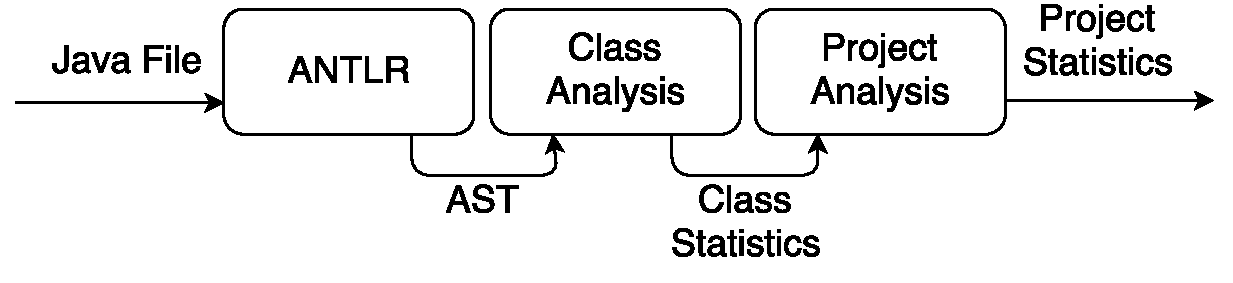
\includegraphics[scale=0.70]{AntlrPipeline.pdf}

The results are then aggregated to produce corpus level analysis which can be found in the following table:
\newline

\captionof{table}{Java Analysis Results}
\begin{tabular}{|l|l|l|l|}
	\hline
	& Count  & \% of classes & \% of extended classes \\ \hline
	Total classes                                                                                   & 116427 &               &                        \\ \hline
	Classes extend another class                                                                    & 71203  & 61.16\%       &                        \\ \hline
	Classes are extended by another class                                                           & 20751  & 17.82\%       &                        \\ \hline
	Classes with forwarding                                                                         & 7087   & 6.09\%        &                        \\ \hline
	\begin{tabular}[c]{@{}l@{}}Classes with forwarding\\ that extend another class\end{tabular}     & 3381   & 2.90\%        &                        \\ \hline
	Classes with downcalls in constructors                                                          & 16101  & 13.83\%       &                        \\ \hline
	Classes storing this in constructors                                                            & 2392   & 2.05\%        &                        \\ \hline
	\begin{tabular}[c]{@{}l@{}}Classes with downcalls or\\ storing this in constructor\end{tabular} & 17099  & 14.69\%       &                        \\ \hline
	\begin{tabular}[c]{@{}l@{}}Extended classes with\\ downcalls in constructors\end{tabular}       & 1545   & 1.33\%        & 7.45\%                 \\ \hline
	\begin{tabular}[c]{@{}l@{}}Extended classes storing\\ this in constructors\end{tabular}         & 178    & 0.15\%        & 0.86\%                 \\ \hline
	Classes with delegation                                                                         & 5183   & 4.45\%        &                        \\ \hline
\end{tabular}

\section{JavaScript}
In JavaScript, there are many ways developers make use of classical inheritance patterns despite the lack of native support in the language. This is largely a result of the numerous libraries which offer their own implementation of classical inheritance behaviour. Some examples of these patterns can be found in the following table:
\captionof{table}{JavaScript Patterns}
\begin{tabular}{|p{5cm}|p{9cm}|}
	\hline
	\multicolumn{2}{|c|}{JavaScript}                                                                                                                                                                  \\ \hline
	Inheritance 1                  & var a = function ( b ) \{    c . call ( this , d );\}                                                                                      \\ \hline
	Inheritance 2                  & function Bar   ( x , y ) \{    Foo . call ( this , x ) ;\}                                                                                 \\ \hline
	Inheritance 3                  & Foo . prototype = object . create ( Bar . prototype )                                                                                      \\ \hline
	Inheritance 4 - Node.js        & var className = defineClass(...)                                                                                                           \\ \hline
	Inheritance 5 - Node.js        & util.inherits(...)                                                                                                                         \\ \hline
\end{tabular}
\newline\newline\newline
The JavaScript analysis in this study makes extensive use of the prior work in developing the JSClassFinder application~\cite{JSClassFinder}. The aim here is to find the cases where JavaScript developers are choosing not to use the native delegation support of the language and are instead modelling their programs with classical inheritance structures. The important factor here is the Class Usage Ratio (CUR) of a JavaScript project as defined in \textit{Does JavaScript Software Embrace Classes?~\cite{JSClassFinder}}. Across a corpus of 50 JavaScript projects, the JSClassFinder returns interesting results about the prevalence of class usage in the language.
\begin{enumerate}
	\item The median CUR across the corpus was 0.15
	\item The upper quartile CUR across the corpus was 0.36
	\item The lower quartile CUR across the corpus was 0.005, which was heavily impacted by 13 systems which had a CUR of zero
\end{enumerate}